%%%%%%%%%%%%%%%%%%%%%%%%%%%%%%%%%%%%%%%%%%%%%%%%%%%%%%%%%%%%%%%%%%%%%%%%%%%%%%
%%Skeleton LaTeX file: double column format.
%%%%%%%%%%%%%%%%%%%%%%%%%%%%%%%%%%%%%%%%%%%%%%%%%%%%%%%%%%%%
%%REMEMBER THAT THERES IS AN EIGHT PAGE SIZE RESTRICTION
%%%%%%%%%%%%%%%%%%%%%%%%%%%%%%%%%%%%%%%%%%%%%%%%%%%%%%%%%%%%

%%% Sample file for ME Project Papers for Evaluation by Supervisor and Reader
\documentclass[twocolumn]{article}
%\documentstyle[twocolumn]{article}
\usepackage{graphicx}
\usepackage{listings}
\usepackage{subfigure}
%\usepackage{caption}
%\usepackage{subcaption}
\pagestyle{empty}
\setlength{\topmargin}{ 0.25in}
\setlength{\columnsep}{2.0pc}
%\setlength{\footheight}{0.0in}
\setlength{\headheight}{0.0in}
\setlength{\headsep}{0.0in}
\setlength{\oddsidemargin}{-.19in}
\setlength{\parindent}{1pc}
\textheight 8.75in
\textwidth 6.8in
\begin{document}
\title{\huge \bf Privacy Preserving Static Analysis }
\author{Soham Ghosh\\Advisor: Prof. Murali Krishna Ramanathan\\Department of Computer Science \& Automation\\Indian Institute of Science} 
\date{$28^{th}$ September, 2013}
\maketitle
\thispagestyle{empty}
%\bibliographystyle{unsrt}
\begin{abstract}
Commercial static analysis tools for software bug detection can discover detects precisely 
but can be expensive monetarily. Open source static analysis tools may not necessarily have 
the precision or depth of their commercial counterparts. Furthermore, deploying static 
analysis tools can add an extra level of complexity to the build process. Changing the usage 
model of static analysis from being a tool to a service can address these issues. In this model, 
a server hosts the static analysis as a service and clients submit their source code to the 
server so that defects can be discovered. However, this approach comes at the cost of revealing 
the source code by the client to the server (a third party). 

In this proposal, we define the problem of {\em privacy preserving static analysis} which 
when addressed can overcome the hurdle associated with revealing the source code. Instead of 
analyzing the original source code, the service analyzes a variant of the original code. 
The first constraint is that the set of defects detected by the analysis on the original source 
or its variant must be the same. The second constraint is that deconstructing the original source code from its variant 
needs to be an arduous task. We address these  two constraints by using {\em code obfuscation} as the 
variant of the original source code. To handle the first constraint, we modify existing 
obfuscation techniques. In order to show that the modifications do not reduce the level of 
obfuscation, we propose a new metric for determining the level of obfuscation (ongoing work). 
 
We will implement our proposal by building a system on top of {\tt ProGuard}, an existing code obfuscator, 
and {\tt FindBugs}, an open source static analysis tool for {\tt Java} programs. We will evaluate our 
implementation by analyzing three large benchmarks {\tt eclipse}, {\tt tomcat} and {\tt lucene}. 
We will show that our implementation addresses the problem of privacy preserving stastic analysis. 
\end{abstract}


\section{Introduction}
Static analysis is used in a number of applications including compilers, tools for program comprehension
and refactoring, tools to verify whether program satisfies certain properties of interest, etc. 
With the increase in size and complexity of codebases of many software systems, static analysis 
has also been adopted to detect bugs effectively~\cite{billionlinesofcode}. Infact, there are a 
number of commercial static analysis tools for software bug detection~\cite{coverity, klocwork, parasoft}. 
These tools are mostly very precise in identifying defects as they are fine tuned based on real-world experiences. 

However, the downside of most commercial tools is that they are expensive. Therefore, it is not always 
feasible for many software developers to get access to these tools. For example, it may not be 
feasible for a mobile application developer to be able to afford these expensive tools. Interestingly, the
number of mobile applications has grown significantly in the recent past and many of them may 
not be able to make their software more reliable due to the expenses involved. 
To address this gap, one can potentially use open source static analysis tools~\cite{findbugs,saturn}. 
However, these tools are not fine tuned to be precise, nor do they encompass the entire gamut of defects 
that need to be detected and they do not have the resources to actively support the users of the tools. 
Therefore, in exchange for using open source tools, software quality is compromised.
Furthermore, irrespective of whether the analysis tool is commerical or not, 
setting them up to be used on a product regularly requires special expertise, resources 
and changes to the build process~\cite{fse13,billionlinesofcode}. 
 
To overcome all these challenges of using a precise and scalable static analysis tool, 
one can envision the use of static analysis as a service. In this usage model, 
the vendors (or developers) of static analysis tools for bug detection provide the tools 
as a service instead of selling them as products. In the presence of a static analysis 
service, product developers (e.g., mobile app developers) can subscribe to the service 
where they are charged on the number of uses. Obviously, using the analysis for a few times 
is relatively inexpensive as opposed to a fixed term license for a product. Furthermore, 
users of the service need not worry about changing their internal build or using other local resources 
to run the static analysis. While this usage model seems appealing at first glance, 
there is a fundamental challenge that needs to be addressed for it to be practical. 
Software organizations (or developers) interested in using static analysis as service 
may not be willing to share their source code with the service provider to ensure 
protection of trade secrets, copy rights and other legal issues. This results in a 
{\em catch-22} situation where the organization cannot share source code with 
a service provider and the service provider cannot detect defects statically without 
the presence of source code. 

In this proposal, we address the problem of building a practical static analysis system 
which can be used as a service without the client revealing its source. To the best 
of our knowledge, we are the first to propose the problem of {\em privacy preserving 
static analysis}. We define privacy preserving static analysis as follows:  

``{\em Given source code $S'$, which is a variant of the original source code $S$, the application of static 
analysis for software bug detection on $S'$ will produce the same set of defects, $D$, 
that is produced by application of the analysis on $S$, and the effort necessary to obtain 
$S$ from $S'$ is non-trivial.}'' 

By this definition of privacy preserving static analysis, if the variant $S'$ is appropriately generated, 
then $S'$ can be used as the input to the static analysis. The user of the analysis needs to 
invest non-trivial amount of effort to decipher the original source $S$ from the variant $S'$. Moreover, 
from the perspective of the user of the analysis, the set of defects detected is exactly the same without 
the cost of revealing the source code. Thus the problem of performing privacy preserving static analysis 
is reduced to the problem of generating a suitable variant of the source code. 

While there can be many approaches to generate the variant, we believe code obfuscation~\cite{collberg} 
fits naturally in this context. Obfuscation is a technique used to transform source code such that
reverse engineering the original source from the obfuscated version is hard. This is a popular 
technique which is widely used~\cite{zelix,jbco,proguard} before deploying a product. A number of 
techniques exist for code obfuscation including control flow obfuscation~\cite{controlflowobf}, 
manufacturing opaque predicates~\cite{collberg}, design obfuscation~\cite{designobf}, etc. 

We design a static analysis system where the {\em client} obfuscates the source code on which defects 
need to be detected and sends it to the {\em server} which hosts the static analysis service. The server 
performs the analysis on the obfuscated code, detects defects and sends the list of 
defects along with supporting data for triaging the defects to the client. To get the defects on the original source code, 
the client maintains a map between the original and obfuscated code and uses this map to transform 
the received defects on obfuscated code into the defects on the original code. 

While the above design satisfies the confidentiality of the source code, it does not necessarily 
satisfy the second property of obtaining the same set of defects. Based on our initial experiments, 
running static analysis~\cite{findbugs} on several large benchmarks~\cite{tomcat,lucene,eclipse} 
and their corresponding obfuscated versions, we observe that the defects detected in the original 
and the obfuscated versions are not {\em exactly} the same. Based on the obfuscation and static analysis techniques 
employed, obfuscation results in the introduction of several new defects being detected which are not 
present in the original code. More interestingly, obfuscation also causes the static analysis to not 
detect defects that exist in the original code which would have been detected by the analysis in the 
absence of obfuscation. To satisfy the second property of obtaining the same set of defects, the underlying 
obfuscation algorithm may need to be appropriately modified. Although the static analysis can also be 
modified but that is not desirable.
 
However, any modification to the underlying obfuscation algorithm raises an important question on whether 
the design compromises on the first property (requiring significant effort for reverse engineering) 
to ensure that the second property is satisfied. For example, it is possible that the modifications 
done to the obfuscation algorithm may make it easier for a malicious server to reverse engineer. 
To address this concern effectively, our approach needs to provide guarantees that the modifications 
do not weaken the first property. In that direction, we need to design a suitable metric to 
measure the level of obfuscation of any source code (ongoing work). 

% our proposed approach does not weaken the obfuscation, we need some metric to compare the obfuscation strength of two obfuscated versions of the same code. Collberg \cite{collberg} 
%measures potent and resilient opaque predicates but in a qualitative way. Some other measures of program obfuscation can relate to instruction count, data-flow, control-flow as 
%distinguished in \cite{sutter} or it may be cyclomatic complexity as mentioned in \cite{McCabe}. Most of the prior works measure code obfuscation qualitatively rather than 
%quantitatively. A very recent work \cite{entropy} suggests on measuring the entropy of an obfuscated code, but unfortunately it only deals with control flow obfuscations. So even such 
%a metric is not enough to compare two obfuscated versions of the same code based on different obfuscation techniques.

%We propose a metric based on graph edit distance to measure code obfuscation. Given a program $P$, 
%a corresponding program dependence graph, $G$, which shows data and control dependencies can 
%be constructed. Similarly, the program dependence graph, $G'$, for the obfuscated version $P'$ of program $P$ 
%can also be constructed. Transforming $G'$ to $G$ is equivalent to obtaining $P$ from $P'$. 
%The problem of transforming one graph to another graph using edit operations (e.g., addition and deletion of 
%edges and nodes) is equivalent to the problem of TODO~\cite{something}. 
%Although this is a NP-Complete problem, but there exist some approximation algorithms such as \cite{Demaine05}. Using 
%these approximation algorithms we can compute the approximate cost of transforming one program dependence graph to its minor. This cost can be assosciated to the cost of reverse 
%engineering and in turn can be used as a metric for code obfuscation.

We propose to incorporate the above design by implementing a privacy preserving static analysis tool. 
The tool will contain a custom-built obfuscator that satisfies the two properties in the definition 
of privacy preserving static analysis. The tool will also include a client-server implementation to handle 
the overall analysis. Finally, we propose to have measurement of the level of obfuscation as a feature of the tool. 
We intend to use {\tt Proguard}~\cite{proguard} as a building block for our custom-built obfuscation and use 
{\tt findbugs}~\cite{findbugs} as the static analysis. 
To evaluate our design and implementation, we will use three benchmark programs -- {\tt eclipse}~\cite{eclipse}, 
{\tt apache-tomcat}~\cite{tomcat} and {\tt apache-lucene}~\cite{lucene}. We will 
show that the set of defects detected on the original and obfuscation versions are identical. 
We will also show that our custom-built obfuscation does not reduce the overall obfuscation. `

We intend to make the following technical contributions: 

\begin{itemize}
\item We are the first to propose the problem of privacy preserving static analysis so that static analysis for
      software bug detection can be used as a service. 
\item We design and implement a privacy preserving static analysis tool. 
\item We propose a novel metric for determining the level of obfuscation -- the cost of reverse engineering. 
\item We will demonstrate the effectiveness of our implementation by analyzing three large benchmarks. 
\end{itemize}
%The rest of the report is structured as follows. In the next section we provide the motivation for the problem along with some examples. Section 3 provides a design overview of privacy 
%preserving static analysis. In section 4 we explain the proposed measure for code obfuscation in details. Finally, in section 5 we present related work and conclude in section 6.

%TODO: Remove the column associated with missing. 
%TODO: Do not scale the box to less than 1. Fix your column length or make the table two columns
\begin{table*}[htb!]
\centering
\scalebox{0.8}{
	\begin{tabular}{| p{5cm} | c | p{7cm} |}
	\hline
	{\tt Checker} & {\tt Count} & {\tt Reason for loss} \\
	\hline
	Method names should start with a lower case letter & 18 & obfuscating with random strings might replace initial uppercase letter of a method with a lowercase character \\
	\hline
	Field is a mutable array & 1 & any method with access to the final array field was pulled out of the class and hence the error does not show anymore \\
	\hline
	Unsynchronized get method, synchronized set method & 2 & getMethod and setMethod get different obfuscated suffix as a result the checker can't compare \\
	\hline
	Should be a static inner class & 36 & inner classes are pulled out during obfuscation \\
	\hline
	Ambigous invocation of either an inherited or outer method & 2 & inner classes are pulled out during obfuscation \\
	\hline
	Class names shouldn't shadow simple name of implemented interface & 2 & classes and interfaces having the same name may get mapped to different random strings \\
	\hline
	Class is not derived from an Exception, even though it is named as such & 2 & classes having exception in their names now get mapped to some random strings \\
	\hline
	Class defines field that masks a superclass field & 1 & fields which had same name as another field in a superclass now get mapped to some random strings \\
	\hline
	\hline
	Total & 64 & \\
	\hline
	\end{tabular}
	}
	\caption{Statistics of defects not detected by {\tt findbugs} after {\tt eclipse}, {\tt tomcat}, {\tt lucene} are obfuscated.}
	\label{tab:missingbugs}
\end{table*} 

\section{Motivation}
In this section, we motivate our proposal further by showing that existing obfuscation are not 
applicable directly. We use examples to show that new defects are detected on the obfuscated version 
that do not existed in the original source. Similarly, defects that exist in the original source 
are masked by the obfuscation. We will briefly provide pointers on how to fix the gain (or loss) 
of defects. 

Table~\ref{tab:missingbugs} shows statistics on the defects that are not detected anymore by {\tt findbugs} on obfuscated 
versions of the three benchmarks. Table~\ref{tab:extrabugs} shows the list of defects 
that are newly detected by {\tt findbugs} due to obfuscation. These defects are not 
detected on the original code. 

%TODO: Remove the column associated with extra. 
%TODO: Do not scale the box to less than 1. Fix your column length or make the table two columns
\begin{table*}[htb!]
\centering
\scalebox{0.8}{
	\begin{tabular}{| p{5cm} | c | p{7cm} |}
	\hline
	{\tt Checker} & {\tt Count} & {\tt Reason for gain} \\
	\hline
	non-transient non-serializable instance field in serializable class & 8 & inner class or even constructors implementing serializable are pulled out as result an object of outer class is created which is non-serializable \\
	\hline
	Class is serializable, but doesn't define serialVersionUID & 14 & in general inner classes are not serializable. But when pulled out they need serialID \\
	\hline
	*Redundant nullcheck of value known to be non-null & 2 & Dataflow analysis cannot decide whether the returned value is null or not in the original code but can determine non-null in obfuscated code \\
	\hline
	Class names should start with an upper case letter & 8 & class names are obfuscated with random strings which may contain a lowercase initial letter \\
	\hline
	Field names should start with a lower case letter & 2 & field names are obfuscated with random strings which may contain a uppercase initial letter \\
	\hline
	Unread public/protected field & 1 & a method which accessed that field might have been moved to another class \\
	\hline
	*Method might ignore exception & 1 & Dataflow analysis can not decide whether an exception may occur or not in the original code but can determine a exception situation in obfuscated code \\
	\hline
	\hline
	Total & 36 & \\
	\hline
	\end{tabular}
	}
	\caption{Statistics of defects newly detected by {\tt articlefindbugs} after {\tt eclipse}, {\tt tomcat}, {\tt lucene} are obfuscated. \newline The exact reason for the gain on the entries
                prefixed with * is to be determined.}
	\label{tab:extrabugs}
\end{table*}

\begin{figure}[ht!]
\centering
\subfigure[Original Program containing the inner class within the outer class]{
       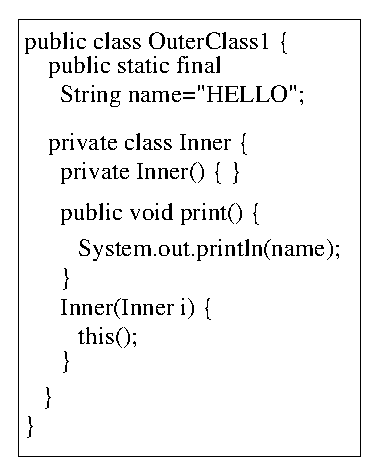
\includegraphics[scale=0.6]{./prog1.eps}
	\label{fig:originnercls}
}
\subfigure[Obfuscated Program with the inner class moved out]{
       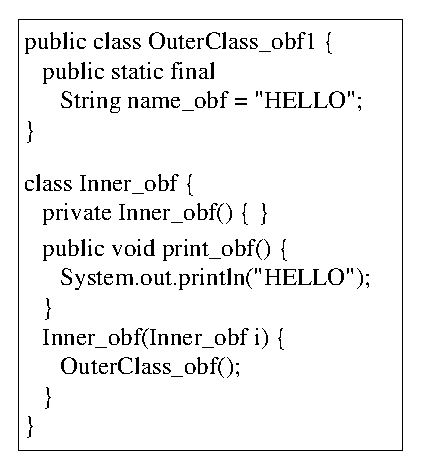
\includegraphics[scale=0.6]{./prog2.eps}
	\label{fig:obfinnercls}
}
\caption{Missing Defects}
\label{fig:missingdefects}
\end{figure}
% \begin{minipage}[t]{0.2\textwidth}
% \lstset{language=Java,captionpos=b,caption={Original Program containing the inner class within the outer class},label=prog:originnercls}
% \begin{scriptsize}
% \begin{lstlisting}
% public class OuterClass {
%  public static final 
%   String name="HELLO";
% 	
%  private class Inner{
%   private Inner(){ }
%   public void print(){
%    System.out.println(name);
%   }
%   Inner(Inner i){
%    this();
%   }
%  }
% }
% \end{lstlisting}
% \end{scriptsize}
% \end{minipage}%
% \hfil\vrule
% \begin{minipage}[t]{0.2\textwidth}
% \lstset{language=Java,captionpos=b,caption={Obfuscated Program with the inner class moved out},label=prog:obfinnercls}
% \begin{scriptsize}
% \begin{lstlisting}
% public class OuterClass_obf {
%  public static final 
%  String name_obf = "HELLO";
% }
%  
% class Inner_obf {
%  private Inner_obf() { }
%  public void print_obf() {
%   System.out.println("HELLO");
%  }
%  Inner_obf(Inner_obf i) {
%   OuterClass_obf();
%  }
% }
% \end{lstlisting}
% \end{scriptsize}
% \end{minipage}%

% \lstset{language=Java,captionpos=b,caption={Original Program containing the inner class within the outer class},label=prog:originnercls}
% \begin{tiny}
% %\tiny
% \begin{lstlisting}[frame=single]
%  public class OuterClass {
% 	public static final String name="HELLO";
% 	
% 	private class Inner{
% 		private Inner(){ }
% 		public void print(){
% 			System.out.println(name);
% 		}
% 		Inner(Inner i){
% 			this();
% 		}
% 	}
% }
% \end{lstlisting}
% \end{tiny}
% %\normalsize
% \lstset{language=Java,captionpos=b,caption={Obfuscated Program with the inner class moved out},label=prog:obfinnercls}
% \begin{tiny}
% \begin{lstlisting}[frame=single]
%  public class OuterClass_obf {
% 	public static final String nkck = "HELLO";
%  }
%  
%  class Inner_obf {
% 	private Inner_obf() { }
% 	public void print_obf() {
% 		System.out.println("HELLO");
% 	}
% 	Inner_obf(Inner_obf i) {
% 		OuterClass_obf();
% 	}
%  }
% \end{lstlisting}
% \end{tiny}
% 
% \lstset{language=Java,captionpos=b,caption={Obfuscated Program with the inner class moved out},label=prog:obfinnercls}
% \begin{tiny}
% \begin{lstlisting}[frame=single]
%  public class OslkrCakrr{
% 	public static final String nkck = "HELLO";
%  }
% 
% class Iiikr{
%     private Iiikr(){ }
%     public void prmia(){
% 	    System.out.println("HELLO");
%     }
%     Iiikr(Iiikr i) {
%       OslkrCakrr();
%     }
%   }
% \end{lstlisting}
% \end{tiny}
% %\normalsize

Now let us look at an example of a missing defect. Figure~\ref{fig:originnercls} shows an example of a defect in the code suggesting that the inner 
class ({\tt Inner}) should be static. But after obfuscation the inner class is moved out of the encompassing ({\tt OuterClass1}) as shown in 
Figure~\ref{fig:obfinnercls} and obfuscated. The result is that the static analysis tool identifies it as a normal class and fails to detect the 
defect that exists in the original code.

Similarly, let us look at an example of an extra defect. Figure~\ref{fig:originnercls1} shows an example in which the outer class is serializable
and has its {\tt serialVersionUID} defined. After obfuscation as shown in Figure~\ref{fig:obfinnercls1}, the inner class is moved outside while making it 
implement the same Serializable class as its outer class. But the obfuscator fails to create a {\tt serialVersionUID} for the inner class. This results in the
introduction of a new defect suggesting that a class that is serializable does not define a {\tt serialVersionUID}.

\begin{figure}[ht!]
\centering
\subfigure[Original Program with the outer class being serializable]{
       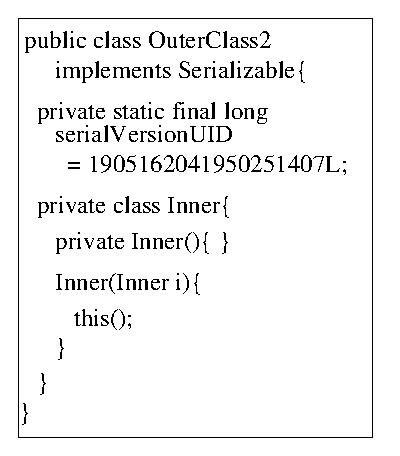
\includegraphics[scale=0.6]{./prog3.eps}
	\label{fig:originnercls1}
}
\subfigure[Obfuscated Program with the inner class being pulled out without having a serialID]{
       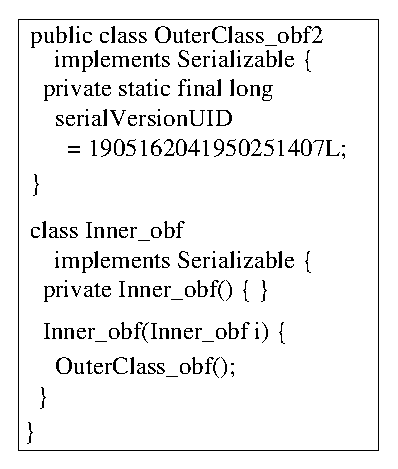
\includegraphics[scale=0.6]{./prog4.eps}
	\label{fig:obfinnercls1}
}
\caption{Extra Defects}
\label{fig:missingdefects}
\end{figure}
% \begin{minipage}[t]{0.2\textwidth}
% \lstset{language=Java,captionpos=b,caption={Original Program containing the inner class within the outer class},label=prog:originnercls1}
% \begin{scriptsize}
% \begin{lstlisting}
% public class OuterClass 
%   implements Serializable{
%     
%   private static final long 
%     serialVersionUID 
%      = 1905162041950251407L;
% 	
%   private class Inner{
%   
%     private Inner(){ }
%     
%     Inner(Inner i){
%       this();
%     }
%   }
% }
% \end{lstlisting}
% \end{scriptsize}
% \end{minipage}%
% \hfil\vrule
% \begin{minipage}[t]{0.2\textwidth}
% \lstset{language=Java,captionpos=b,caption={Obfuscated Program with the inner class moved out},label=prog:obfinnercls1}
% \begin{scriptsize}
% \begin{lstlisting}
% public class OuterClass_obf 
%   implements Serializable {
%     
%   private static final long 
%     serialVersionUID 
%      = 1905162041950251407L;
% }
% 
% class Inner_obf 
%   implements Serializable {
%     
%   private Inner_obf() { }
%   Inner_obf(Inner_obf i) {
%     OuterClass_obf();
%   }
% }
% \end{lstlisting}
% \end{scriptsize}
% \end{minipage}%

% \begin{minipage}[t]{0.2\textwidth}
% \lstset{language=Java,captionpos=b,caption={Original Program with the outer class being serializable},label=prog:originnercls1}
% \begin{tiny}
% \begin{lstlisting}
% public class OuterClass 
%     implements Serializable{
%     
%     private static final long 
%     serialVersionUID 
%       = 1905162041950251407L;
% 	
%     private class Inner{
% 	private Inner(){
% 	}
% 	Inner(Inner i){
% 	    this();
% 	}
%     }
% }
% \end{lstlisting}
% \end{tiny}
% \end{minipage}%
% \hfill\vrule\hfill
% \begin{minipage}[t]{0.2\textwidth}
% \lstset{language=Java,captionpos=b,caption={Obfuscated Program with the inner class being pulled out without having a serialID},label=prog:obfinnercls1}
% \begin{tiny}
% \begin{lstlisting}
% public class OuterClass_obf 
%     implements Serializable {
%     
%     private static final long 
%     serialVersionUID 
%       = 1905162041950251407L;
% }
% 
% class Inner_obf 
%     implements Serializable {
%     
%     private Iiikr() { }
%     Iiikr(Iiikr i) {
% 	OslkrCakrr();
%     }
% }
% \end{lstlisting}
% \end{tiny}
% \end{minipage}%

A simple solution for the extra defects problem in Figure~\ref{fig:originnercls1} and Figure~\ref{fig:obfinnercls1} is to make the inner class non-serializable
while moving out. But this is not always possible as the innerclass may access some serial fields of the outerclass. 
\begin{figure}[ht!]
\centering
\subfigure[Solution to missing defect in Figure~\ref{fig:obfinnercls}]{
       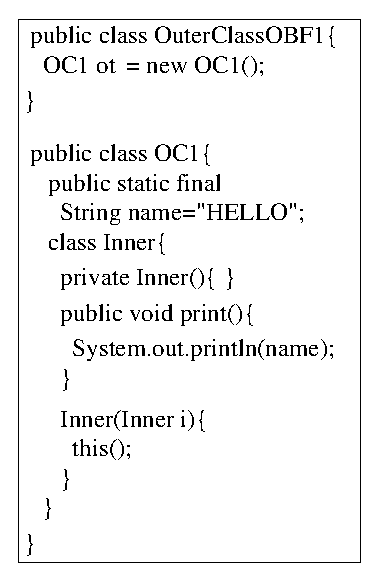
\includegraphics[scale=0.6]{./prog5.eps}
	\label{fig:originnercls2}
}
\subfigure[Solution to extra defect in Figure~\ref{fig:obfinnercls1}]{
       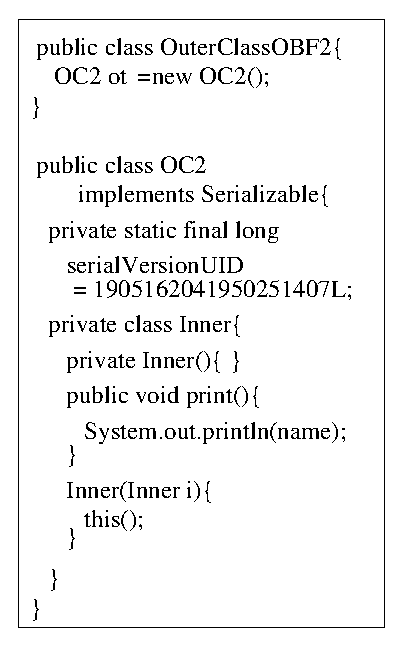
\includegraphics[scale=0.6]{./prog6.eps}
	\label{fig:obfinnercls2}
}
\caption{Solution addressing the extra and missing defects}
\label{fig:missingdefects}
\end{figure}
% \begin{minipage}[t]{0.2\textwidth}
% \lstset{language=Java,captionpos=b,caption={Solution to missing defect in Listing~\ref{prog:obfinnercls}},label=prog:obfinnercls2}
% \begin{scriptsize}
% \begin{lstlisting}
% public class OuterClass_obf{
%   OuterClass1 ot
%     = new OuterClass1();
% }
%  
% public class OuterClass1{
%  public static final 
%   String name="HELLO";
% 	
%  class Inner{
%   private Inner(){ }
%   
%   public void print(){
%    System.out.println(name);
%   }
%   
%   Inner(Inner i){
%    this();
%   }
%  }
% }
% \end{lstlisting}
% \end{scriptsize}
% \end{minipage}%
% \hfil\vrule
% \begin{minipage}[t]{0.2\textwidth}
% \lstset{language=Java,captionpos=b,caption={Solution to extra defect in Listing~\ref{prog:obfinnercls1}},label=prog:obfinnercls3}
% \begin{scriptsize}
% \begin{lstlisting}
% public class OuterClass_obf{
%  OuterClass1 ot
%    =new OuterClass1();
% }
%  
% public class OuterClass2
%  implements Serializable{
%  
%  private static final long 
%    serialVersionUID 
%     = 1905162041950251407L;
%      
%  private class Inner{
%   private Inner(){ }
%   public void print(){
%    System.out.println(name);
%   }
%   Inner(Inner i){
%    this();
%   }
%  }
% }
% \end{lstlisting}
% \end{scriptsize}
% \end{minipage}%

A possible solution to the missing defects problem is to obfuscate the code as given in Figure~\ref{fig:originnercls2}. 
The entire content inside the original encompassing class, {\tt OuterClass1} of Figure~\ref{fig:originnercls}, including the innerclass {\tt Inner} is moved to a newly 
created class named {\tt OC1}. Basically {\tt OC1} is a copy of the old {\tt OuterClass1} (in Figure~\ref{fig:originnercls}. 
The obfuscated version of the {\tt OuterClass1} ({\tt OuterClassOBF1}) now contains only an object of {\tt OC1}, using which it can 
access all its old data members and methods. 

Similarly, for the extra defect problem a possible solution is to obfuscate the code as given in Figure~\ref{fig:obfinnercls2}. 
Like in the previous solution, the entire content inside the original encompassing class {\tt OuterClass2} of Figure~\ref{fig:originnercls1}, 
including the innerclass {\tt Inner} is moved to a newly created class named {\tt OC2}. Basically {\tt OC2} is a copy of the old {\tt OuterClass2} 
(in Figure~\ref{fig:originnercls1}). The obfuscated version of the {\tt OuterClass1} ({\tt OuterClassOBF2}) now contains only an object of {\tt OC2}, 
using which it can access all its old data members and methods. 

In the above two solutions, all the data accesses and function calls of the old outer class is redirected through an object of this new class. Since the suggested technique is built 
on top of the existing obfuscation technique, it actually makes the existing obfuscation technique more stringent. We also observe that defects are neither lost nor 
gained for the Figure\ref{fig:originnercls} and Figure\ref{fig:originnercls1}.

The examples shown in this section provide a brief overview of the problems that are encountered while running static analysis on obfuscated programs. Furthermore it is not clear 
whether the modified obfuscation actually increases or decreases the level of obfuscation, even though we claim that it has increased. Therefore instead of a subjective argument, 
an objective metric to determine the level of obfuscation will be helpful. This motivates the design of the obfuscation metric.
\section{Architecture Overview}
The overall system architecture of Privacy Preserving Static Analysis is shown in Figure \ref{fig:architecture}. We broadly divide the system into three major components: 
{\tt Obfuscator}, {\tt SA Server} and {\tt Remapper}. An additional unit {\tt Obfuscation Evaluator} measures the strength of obfuscation.

\begin{figure}[h]
 \centering
 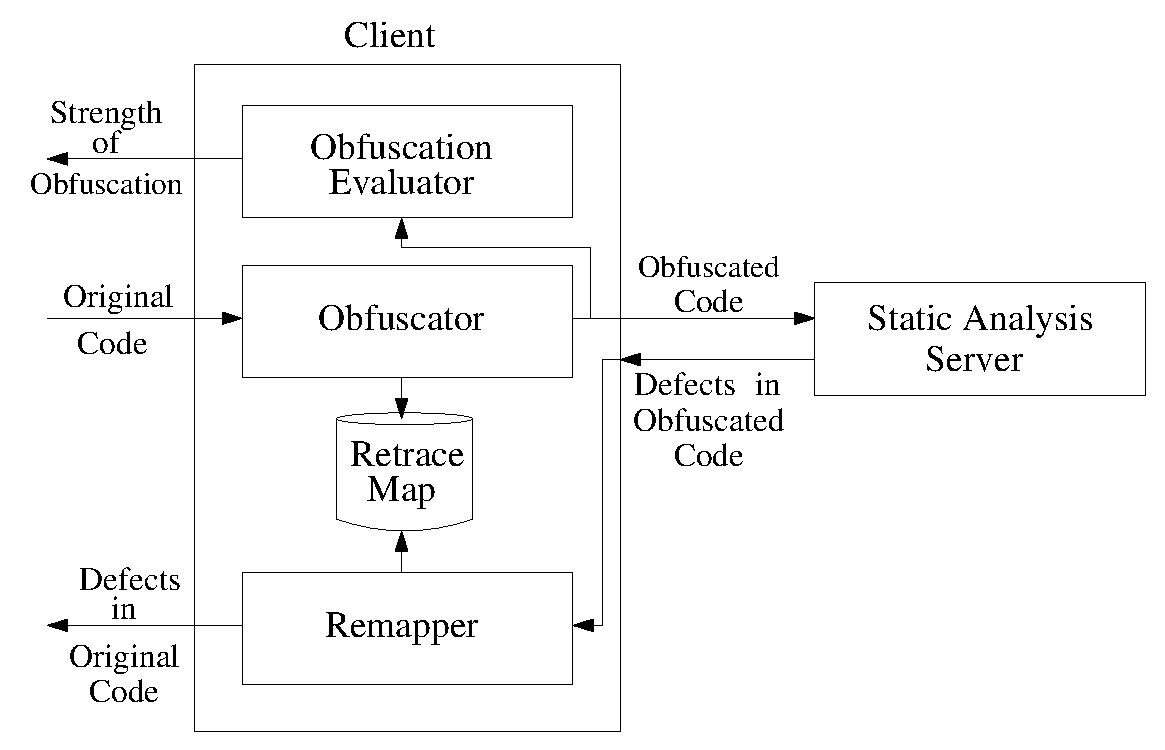
\includegraphics[scale=0.4]{./architecture2.eps}
 % architecture.eps: 0x0 pixel, 300dpi, 0.00x0.00 cm, bb=
 \caption{Architecture of the Privacy Preserving Static Analysis System}
 \label{fig:architecture}
\end{figure}

{\tt Obfuscator} takes as input the original unobfuscated source code and applies certain obfuscation techniques to produce an obfuscated version of the source code, which 
ensures that no new defects are introduced and none of the old defects are missing in the obfuscated code. During this obfuscation process our tool also produces a {\tt Retrace Map} which maintains a 
mapping of obfuscated package, class, method and variable names to their original ones. The map also stores the full classpath for each and every item in case of repackaging of classes 
or inner classes being moved out of their outer classes. For our system we use {\tt Proguard}~\cite{proguard} as the basis for obfuscation. We modify the existing obfuscation 
techniques in Proguard to guarantee the preservation of defects.

The obfuscated code is then sent to the {\tt SA Server}. The SA Server runs several static analysis techniques on the obfuscated code and reports back a 
list of detected defects. At this stage even if someone tries to reverse engineer the received code, it will be a non-trivial task. In this project, 
we are using {\tt FindBugs}~\cite{findbugs} to perform the static analysis.

The defect summary for the obfuscated code is then sent back to the client, where it is passed through the {\tt Remapper}. The {\tt Remapper} remaps the defects in the obfuscated code to 
the respective defects in the original code. It does so by using the contents of the {\tt Retrace Map} produced during the obfuscation phase, and then replaces each obfuscated name, line number 
and classpath with the original values . In the end it produces the defect summary for the original code.

Another essential part of the tool is the {\tt Obfuscation Evaluator}. It takes as input both the original and obfuscated code and then measures the strength of obfuscation (ongoing work).
% The tool 
% creates the program dependency graph for both the original and obfuscated program, say $G$ and $G'$ respectively. Now using approximation algorithms for solving {\tt Graph Minor} 
% \cite{graphminor} problem, it calculates the cost of transforming $G'$ to $G$. This cost gives an estimate of the cost of reverse engineering, and in turn gives a measure for the 
% strength of code obfuscation. We explain {\tt Obfuscation Evaluator} in detail in the next subsection.

%\subsection{Measurement of Obfuscation}
%In this section we are going to explain in detail the proposed method for measuring the strength of obfuscation including the logic behind it, using examples and step by step procedure 
%for calculating the strength of obfuscation. We can represent any program using a {\tt Program Dependence Graph}, which represents both control and data dependencies. Any obfuscation 
%technique increases the complexity level of control flow and data dependencies, and any reverse engineering process tries to simplify them. Therefore it seems very natural to argue about 
%the strength of obfuscation using program dependence graph. So in terms of dependence graphs the process of reverse engineering can be seen as a transformation of the obfuscated dependence 
%graph to the original dependence graph. We will show this using the following example.
%\lstset{language=Java,captionpos=b,caption={Original Code for squaring},label=prog:origsqr}
%\tiny\begin{lstlisting}[frame=single]
% int square(int x){
%	  int n;
%	  n = x * x;
%	  return n;
%  }
%\end{lstlisting}
%\normalsize
%\lstset{language=Java,captionpos=b,caption={Obfuscated Code for squaring},label=prog:obfsqr}
%\tiny\begin{lstlisting}[frame=single]
% int strvup(int m){
%	  int o;
%	  int i=0;
%	  int s=0;
%	  while(i < m){
%		   s = s + m;
%		   i = i + 1;
%	  }
%	  o = s;
%	  return s;
% }
%\end{lstlisting}
%\normalsize
%Listing \ref{prog:origsqr} represents a code to calculate the square of a number and Listing \ref{prog:obfsqr} represents the obfuscated version of it. The corresponding program dependency 
%graphs are shown in Figure \ref{fig:origsqr} and Figure \ref{fig:obfsqr1}.
%\begin{figure}[h]
% \centering
% 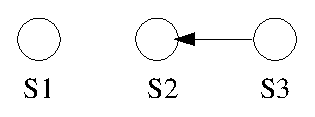
\includegraphics[scale=0.3]{./origdep.eps}
% % architecture.eps: 0x0 pixel, 300dpi, 0.00x0.00 cm, bb=
% \caption{Program dependence graph for Listing \ref{prog:origsqr}}
% \label{fig:origsqr}
%\end{figure}
%\begin{figure}[h]
% \centering
% 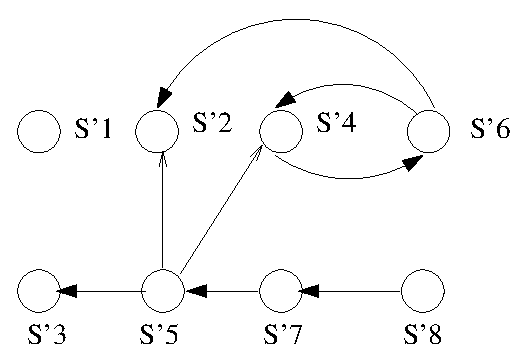
\includegraphics[scale=0.3]{./obfdep1.eps}
% % architecture.eps: 0x0 pixel, 300dpi, 0.00x0.00 cm, bb=
% \caption{Program dependence graph for Listing \ref{prog:obfsqr}}
% \label{fig:obfsqr1}
%\end{figure}
%
%Transforming the graph in Figure \ref{fig:obfsqr1} to that in Figure \ref{fig:origsqr} requires a series of operations such as: {\tt edge and node deletion}, and {\tt edge contraction}. 
%The sequence of steps needed are shown in Figures \ref{fig:obfsqr2} to \ref{fig:obfsqr7}.
%\begin{figure}[ht!]
% \centering
% \subfigure[Step 1]{
%        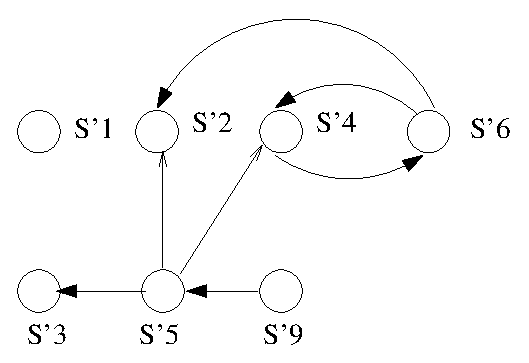
\includegraphics[scale=0.28]{./obfdep2.eps}
%	\label{fig:obfsqr2}
% }
% \subfigure[Step 2]{
%        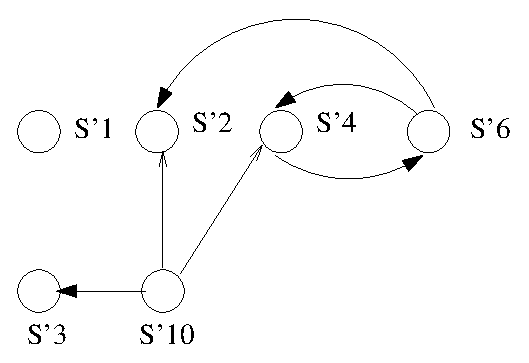
\includegraphics[scale=0.28]{./obfdep3.eps}
%	\label{fig:obfsqr3}
% }
% \subfigure[Step 3]{
%        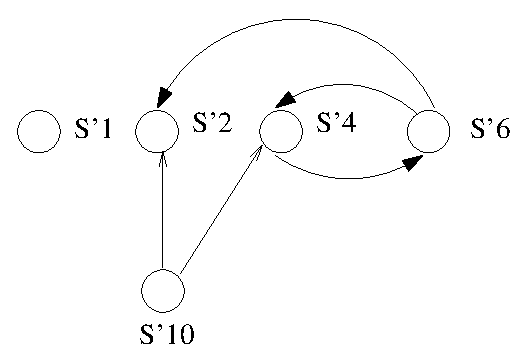
\includegraphics[scale=0.28]{./obfdep4.eps}
%	\label{fig:obfsqr4}
% }
% \\
% \subfigure[Step 4]{
%        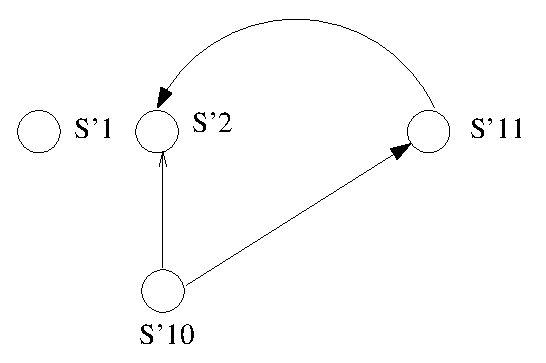
\includegraphics[scale=0.3]{./obfdep5.eps}
%	\label{fig:obfsqr5}
% }
% \subfigure[Step 5]{
%        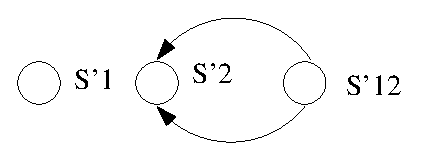
\includegraphics[scale=0.3]{./obfdep6.eps}
%	\label{fig:obfsqr6}
% }
% \subfigure[Step 6]{
%        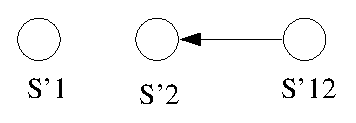
\includegraphics[scale=0.3]{./obfdep7.eps}
%	\label{fig:obfsqr7}
% }
%\caption{Transformation Steps}
%\label{fig:transfrm}
%\end{figure}
%From Figures \ref{fig:obfsqr2} to \ref{fig:obfsqr7} we see that 4 edge contractions and 2 edge and node deletion is required. During the process of reverse engineering we see that merging 
%of two statements is more costlier than deletion of a statement. Hence we can assign higher weightage to edge contraction operations in comparison to edge and node deletion operations. 
%We assign each edge contraction operation a weight of 2 and each edge and node deletion operation a weight of 1. Using these weights the cost of reverse engineering or analogously the 
%strength of obfuscation is: $4 * 2 + 2 * 1 = 10$.
%% \begin{figure}[h]
%%  \centering
%%  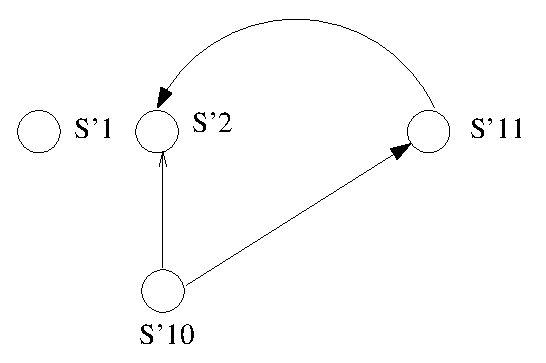
\includegraphics[scale=0.3]{./obfdep5.eps}
%%  % architecture.eps: 0x0 pixel, 300dpi, 0.00x0.00 cm, bb=
%%  \caption{Step 4}
%%  \label{fig:obfsqr5}
%% \end{figure}
%% \begin{figure}[h]
%%  \centering
%%  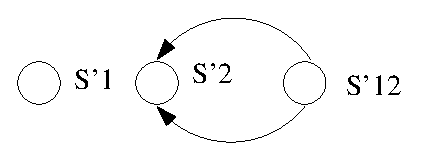
\includegraphics[scale=0.3]{./obfdep6.eps}
%%  % architecture.eps: 0x0 pixel, 300dpi, 0.00x0.00 cm, bb=
%%  \caption{Step 5}
%%  \label{fig:obfsqr6}
%% \end{figure}
%% \begin{figure}[h]
%%  \centering
%%  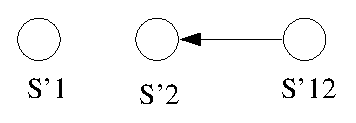
\includegraphics[scale=0.3]{./obfdep7.eps}
%%  % architecture.eps: 0x0 pixel, 300dpi, 0.00x0.00 cm, bb=
%%  \caption{Step 6}
%%  \label{fig:obfsqr7}
%% \end{figure}
%This method of transforming one graph to another can be mapped to a very popular problem in Graph Theory, known as Graph Minor \cite{graphminor}. Dtermining the steps required for the 
%transformation to find the Graph Minor is a NP-Complete problem. But there exist approximation algorithms \cite{Demaine05} for this, using which we can get the approximate steps required. 
%Once we have knowledge of these steps, we can then calculate the strength of obfuscation using the above weights for any pair of original and obfuscated code.



\section{Related Work}
\subsection{Preserving Privacy Techniques}
The concept of privacy preserving static analysis and the idea of providing static analysis is completely new and as such there has been no prior work in this field. The work closest 
to our own is CryptDB project~\cite{cryptdb}, which is in the field of database systems. CryptDB uses homomorphic encryption to run secured queries on relational databases. It applies 
the encryption schemes on the data in a sequential manner. The SQL queries are analysed on the fly, and the data columns 
are decrypted to the required encryption layers to execute the query on the server. 

In the field of program analysis, MrCrypt~\cite{mrcrypt} uses the similar concept of homomorphic 
encryption to securely execute programs on cloud servers without revealing input data. MrCrypt performs type inferencing on a program to identify the set of operations applied on each input data 
column, and appropriately chooses a homomorphic encryption scheme for that column. The data columns are encrypted and the program is also transformed accordingly to operate over 
the encrypted data. The encrypted data and transformed program are then sent to the server for execution, and the encrypted result of the computation is decrypted on the client side. 
Both these approaches concentrate on encrypting program data rather than hiding the program structure itself. Moreover the idea of encryption cannot be applied for securing 
program structures as it is not possible to run static analysis on encrypted program semantics. So in our proposed method of privacy preserving static analysis, obfuscation of code 
successfuly hides program structure without caring about program data, while keeping the program semantics unchanged.

Applied largely in the field of cryptography, Zero-Knowledge proofs play an important role in privacy preservation. Goldwasser et al.~\cite{Goldwasser} conceived the idea of ZKPs 
and suggested the concept of knowledge complexity, a measurement of the amount of knowledge about the proof transferred from the prover to the verifier. Goldreich et al.~\cite{Goldreich} 
constructs a ZKP for the graph three-colorability problem and then further extends the proof to show that there exists a ZKP for any language in NP. The Fiege-Fiat-Shamir identification 
scheme~\cite{Fiege} is the basis of most zero-knowledge indetification protocols currently in use in the domain of cryptography.

\subsection{Static Analysis}
There has been substantial work in using static analysis to find bugs in programs. Dillig et al.~\cite{dillig} propose a technique to precisely compute neccessary and sufficient 
conditions required by program points that are path-sensitive and context-sensitive.Instead of collecting abstract specifications that are then verified by model checkers like 
SPIN~\cite{spin} or theorem provers like Z3~\cite{z3}, Engler et al.~\cite{engler} propose an approach using metalevel compilation ({\tt MC}) to automatically check system rules. 
Today several tools exist in the market which provide 
static analysis to detect bugs~\cite{coverity,klocwork,parasoft,findbugs,chess,saturn}. FindBugs \cite{findbugs} uses bug pattern detectors to find real bugs in several real world 
Java applications and libraries. Our tool uses FindBugs to perform the task of static analysis. But any other tool detecting defects would also work fine, since in our tool we 
modified the obfuscation techniques based on certain properties of defect checkers, and not the implementation of the analysis itself.

\subsection{Obfuscation Techniques}
There has been a lot of prior work in the field of code obfuscation. An initial theoretical approach to obfuscation is presented by Collberg et al.~\cite{collberg}. 
They introduce the concepts of lexical obfuscation (random strings used for naming) and data transformations (such as obtaining a boolean value at evaluation time from the combination 
of two distinct expressions). However, their chief contributions are in control-flow obfuscation. They exploit the difficulty of analyzing aliases and concurrent programs to 
construct opaque predicates. Wang et al.~\cite{wang} suggests combining the data of a program with its control-flow and thereby making control and data flow analysis interdependent. 
Sakabe et al.~\cite{sakabe} concentrate their efforts on the object-oriented nature of Java. Using polymorphism, they invent a universal datatype class to encapsulate all return types 
and method parameters thus hidding their true types. Sonsonkin et al.~\cite{sonsonkin} attempt to confuse program structure by combining multiple class files into one. For our system 
we are building on top of Proguard tool~\cite{proguard} and can use any of the suitable obfuscation technique.

\subsection{Measure of Obfuscation}
Although there have been several approaches related to code obfuscation, we are unaware of any work for measuring obfuscation strength. Collberg et al. 
\cite{collberg} measures potent and resilient opaque predicates but in a qualitative way. Some other measures of program obfuscation relate to instruction count, data-flow, 
control-flow as discussed in~\cite{sutter} or it may be cyclomatic complexity as mentioned in~\cite{McCabe}. Most approaches measure code obfuscation qualitatively rather 
than quantitatively. A very recent work~\cite{entropy} suggests measuring the entropy of an obfuscated code, but unfortunately it only deals with control flow obfuscation. We will deal 
with these problems in our project by defining a new metric for measuring the strength of obfuscation (ongoing work).
% proposed method by representing programs as program dependence graphs, and then draw an analogy between reverse engineering and transformation of obfuscated 
% dependence graph to original dependence graph. Although this is a NP-Complete problem, but there exist some approximation algorithms such as~\cite{Demaine05}. Using these approximation 
% algorithms we can compute the approximate cost of reverse engineering.
%%%%%%%%%%%%%  This can be followed by several other sections

% \section{Conclusions}
% We present the notion of privacy preserving static analysis system and the design for its implementation. The project is the first of its kind to define static analysis as a service, 
% but at the same time it also preserves the privacy of the analysed programs. We want to define a measure for calculating and comparing the strength of obfuscated codes, which gives the 
% true cost of reverse engineering. We will implement all these as a part of a tool which takes a program as input and outputs the obfuscated version of it such that, it preserves all 
% the defects. The tool will also report a value indicating the strength of the obfuscated code. The effectiveness of the tool will be verified by running it on the three large benchmark 
% programs.
\bibliography{citation}
\bibliographystyle{plain}
\end{document}


